\section*{Introduction}\index{Hexapoda}
Here we begin looking at taxa classified in \textbf{Hexapoda}. In most cases you will examine multiple families, most of which you will be tested on in lab practicals. You may be shown more families than are in this manual---primarily so that you can better grasp the diversity that exists---but you will not have to sight-identify these other families. Looking at these other families may help to you, though, in identifying specimens for your collection. Some characters might be impossible to see, given the equipment and specimens we have in lab, but they are provided for future reference.

\section{Hexapoda}

\begin{itemize}
\item 3 tagmata present: head, thorax, abdomen
\item 3 pairs of uniramous thoracic appendages (legs) present
\end{itemize}

\section*{Entognatha}\index{Entognatha}

\begin{itemize}
\item Antennae, when present, truly segmented (\textit{i.e.}, each segment has intrinsic musculature; see figure \ref{fig:dipluraAntenna})
\item Mouthpart concealed externally (figure \ref{fig:proturans}, left)
\item Tarsus not subdivided into tarsomeres (figure \ref{fig:proturans}, right)
\end{itemize}

\begin{figure}[ht!]
    \centering
    \begin{subfigure}[ht!]{0.2\textwidth}
        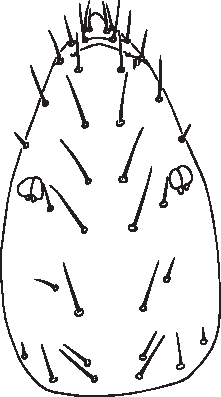
\includegraphics[width=\textwidth]{nonpterygote/proturanHead}
        \caption{}
        \end{subfigure}
    \hfill
    \begin{subfigure}[ht!]{0.12\textwidth}
        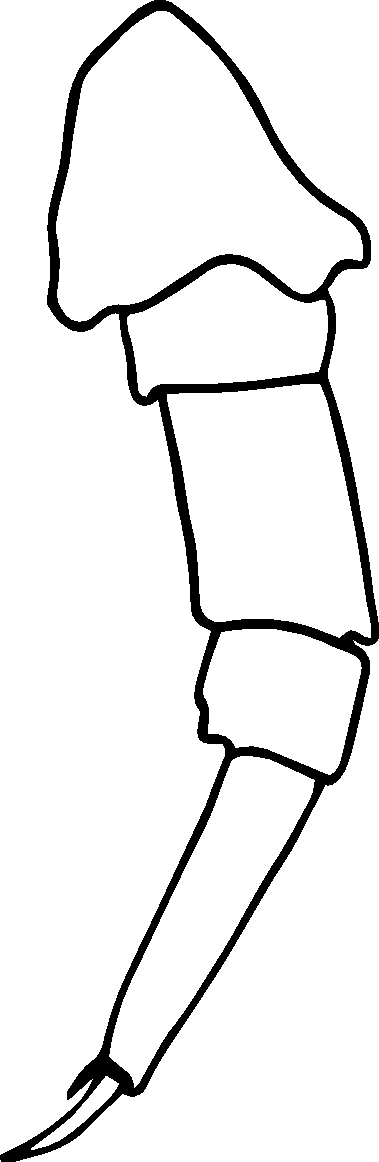
\includegraphics[width=\textwidth]{nonpterygote/proturanLeg}
        \caption{}
    \end{subfigure}
    \caption{Protura. \textbf{(a)} Head in dorsal view, with pseudoculi \citep[][Fig. 1A]{Yun2016}; \textbf{(b)} Leg \cite[redrawn from][Fig. 12]{bhlpart35427}}\label{fig:proturans}
\end{figure}

\subsection{Protura (coneheads)}\index{Protura}
\noindent{}\textit{Diagnostic characters:} Antennae apparently absent (figure \ref{fig:proturanhab}); eyes absent; sensory organs (pseudoculi) present where one would expect eyes or antennae to be; mandibles without molar area (proximal flattened region for grinding food); body very small (\textless1.5 mm long); abdomen 11-segmented in mature specimens, cerci absent.\vspace{3mm}

\noindent{}\textit{Natural History:} Proturans can be abundant in leaf litter and soil samples, but they are incredibly small and usually overlooked. More than 800 species have been described worldwide, and most are smaller than 1 mm.\vspace{3mm}

\begin{theo}
{}How might the absence of antennae be adaptive for these hexapods? Which structure functions as the primary anterior sensory appendage? \end{theo}\vspace{3mm}

\begin{figure}[ht!]
  \centering
    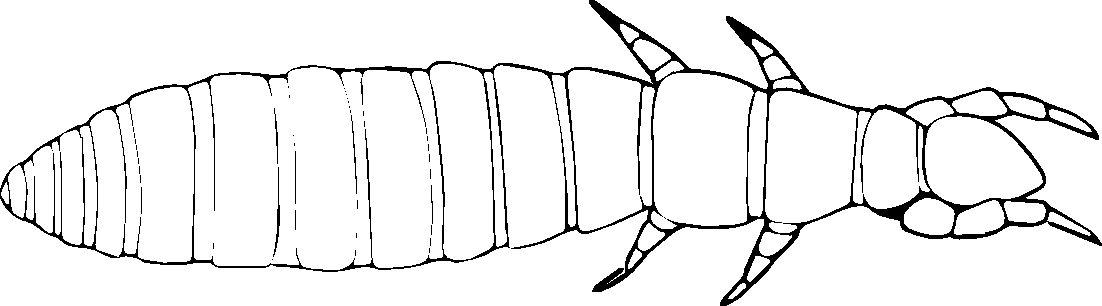
\includegraphics[width=0.55\textwidth]{nonpterygote/proturaHabitus}
  \caption{Protura habitus (illustration by Laura Porturas, Penn State)}
  \label{fig:proturanhab}
\end{figure}

\subsection{Diplura (diplurans)}\index{Diplura}
\noindent{}\textit{Diagnostic characters:} Antennae filiform; eyes absent; pseudoculi absent; mandibles without molar area; body usually \textgreater3 mm long; cerci distinct; abdominal segments often with styli.\vspace{3mm}

\noindent{}\textit{Natural History:} These hexapods are quite common, especially under rocks and logs, at the interface between leaf litter and soil. Like Protura, there are approximately 800 species known worldwide, but diplurans are generally much larger (up to 5 mm long in North America and up to 5 cm in the tropics).\vspace{3mm}

\begin{theo}
{}Compare \textbf{Japygidae} (figure \ref{fig:japygidhab}) to \textbf{Campodeidae} (figure \ref{fig:campodeidhab}). What is your hypothesis for why the cerci vary phenotypically between families? What is their function?\end{theo}

\begin{figure}[ht!]
  \centering
    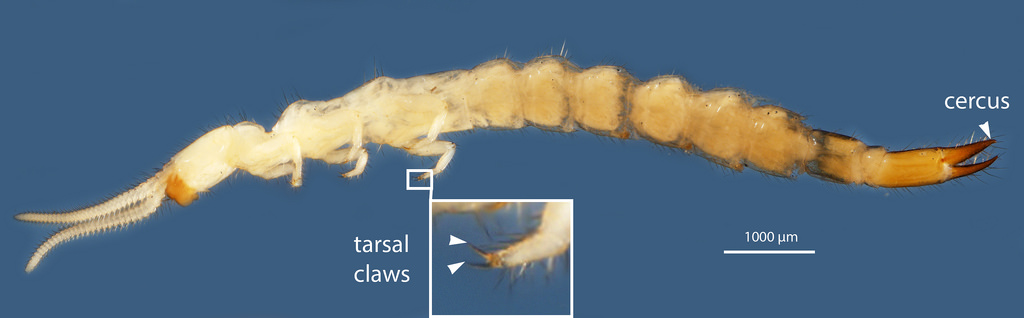
\includegraphics[width=0.6\textwidth]{nonpterygote/japygid1}
  \caption{Japygidae dorsal habitus (illustration by Laura Porturas, Penn State)}
  \label{fig:japygidhab}
\end{figure}
\begin{figure}[ht!]
  \centering
    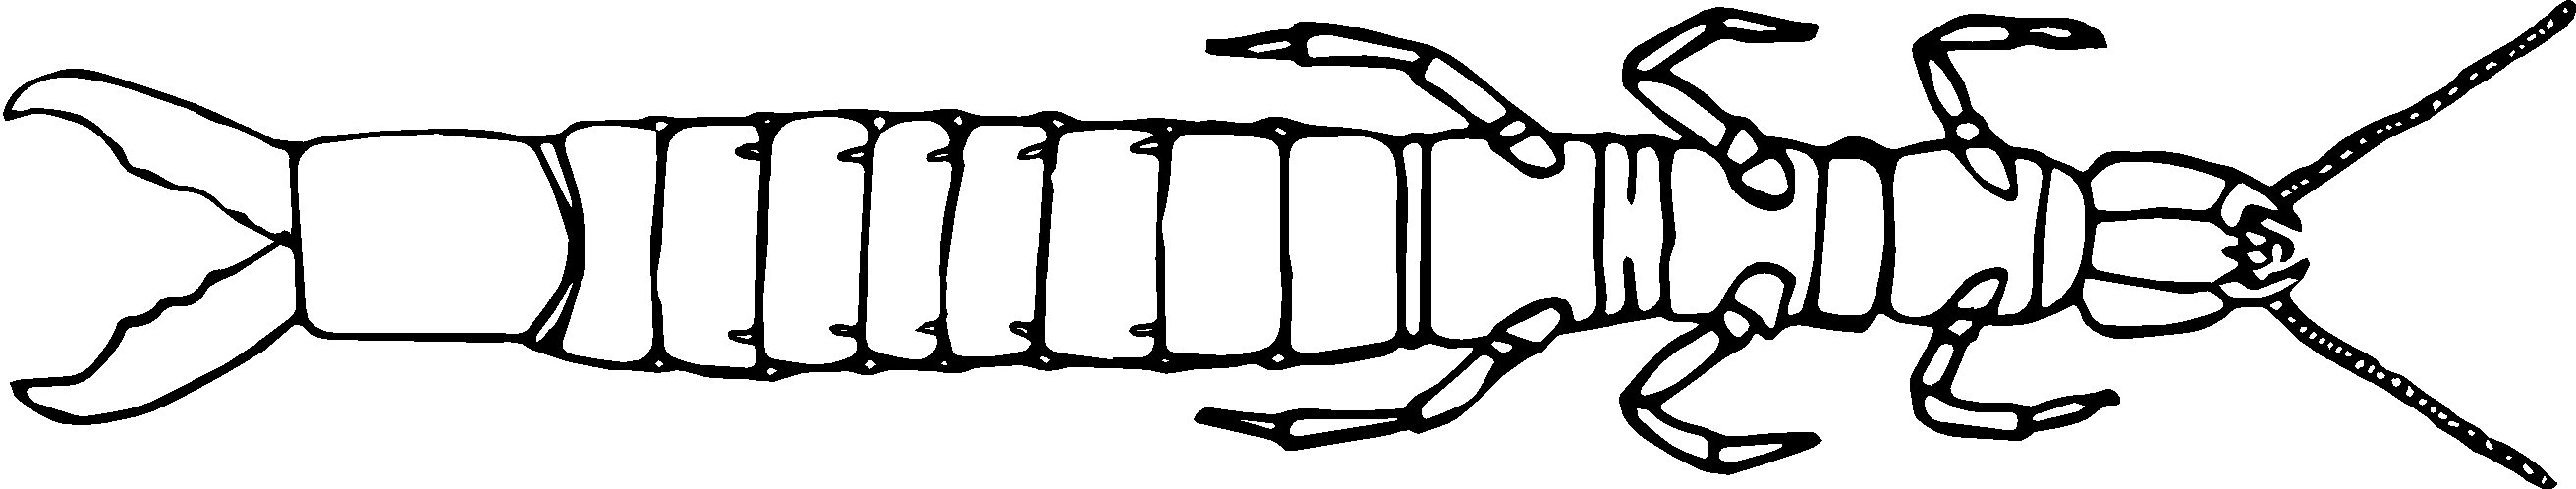
\includegraphics[width=0.6\textwidth]{nonpterygote/DipluraVentral}
  \caption{Japygidae ventral habitus \citep[redrawn from][Fig. 8]{bhlitem30465Insects}}
  \label{fig:japygidhabvent}
\end{figure}

\begin{figure}[ht!]
  \centering
    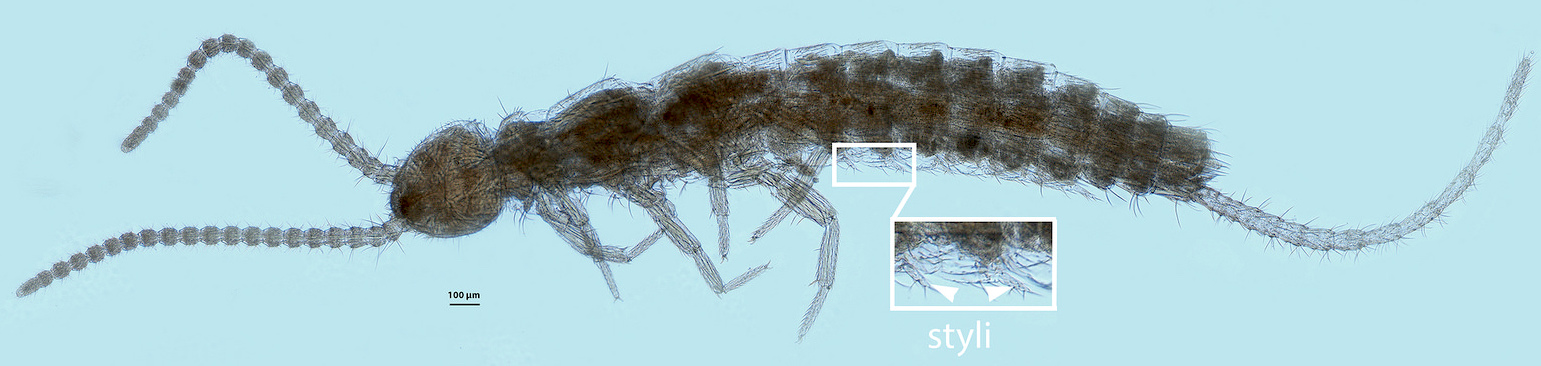
\includegraphics[angle=270,width=0.6\textwidth]{nonpterygote/campodeid1}
  \caption{Campodeidae habitus (illustration by Laura Porturas, Penn State)}
  \label{fig:campodeidhab}
\end{figure}

\begin{figure}[ht!]
  \centering
    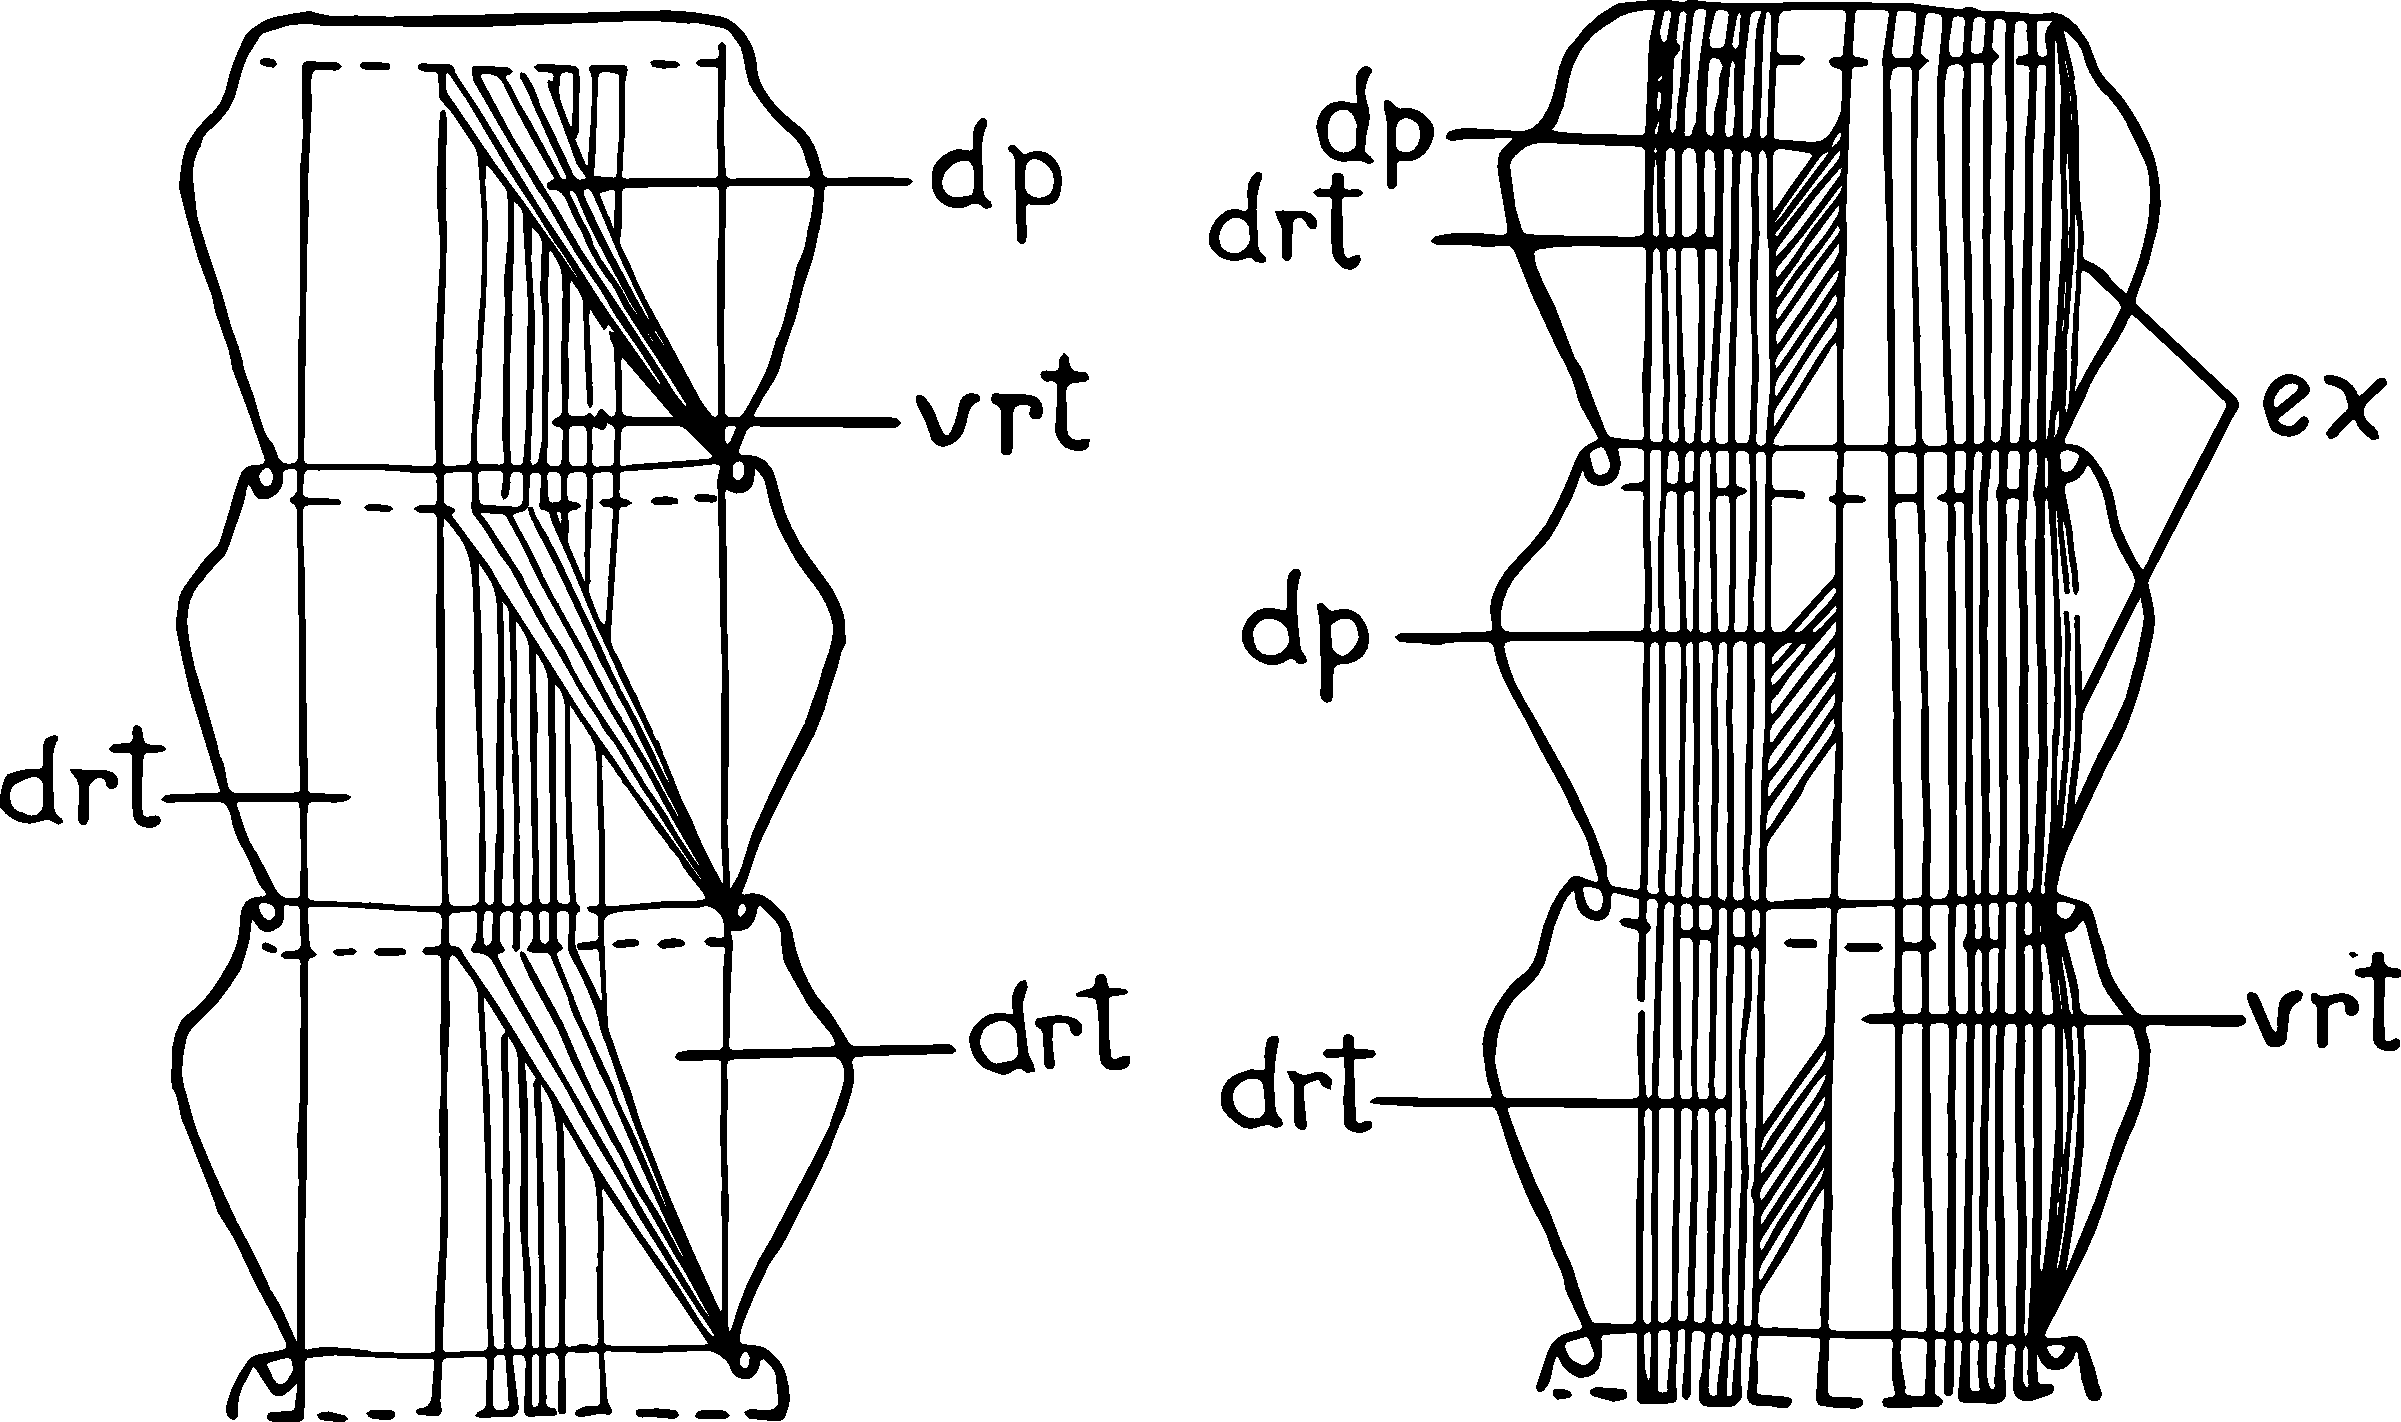
\includegraphics[width=0.5\textwidth]{nonpterygote/dipluraAntenna}
  \caption{Diplura antenna. Antennal segments VIII to X of a species of \textit{Japyx}; left, ventral view; right, dorsal view; dp, depressor muscle; drt, dorsal retractor muscle; ex, extensors; vrt, ventral retractor muscle \citep[redrawn from][Fig. 2]{bhlpart81512}}
  \label{fig:dipluraAntenna}
\end{figure}

\subsection{Collembola (springtails)}\index{Collembola}
Collembola are commonly referred to as ``springtails'' for their ability to jump using a structure called a \latinword{furculum}. We will focus on higher-level taxa, which are usually ranked as orders: Symphypleona, Poduromorpha, Entomobryomorpha. Collembola can be recognized by the following traits:

\begin{itemize}
\item Compound eyes present
\item mandibles with molar area
\item antennae usually $\leq$4 segments
\item tibia fused with tarsus (tibiotarsus)
\item abdomen with $\leq$6 segments: 1st segment with ventral tube (collophore), 3rd abdominal segment modified ventrally (retinaculum) to receive furculum, 5th abdominal segment with forked structure (furculum), usually folded under abdomen
\item body length usually 1--3 mm
\end{itemize}

\subsubsection{Symphypleona (globular springtails)}\index{Symphypleona}
\noindent{}\textit{Diagnostic characters:} Head typically hypognathous, anteroposteriorly flattened; antennae longer than head; prothorax indistinct dorsally, narrowly articulated with head; several abdominal segments fused dorsally.\vspace{3mm}

\noindent{}\textit{Natural History:} Biologically diverse. Symphypleona is subdivided into about 10 families. Some species are semiaquatic.\vspace{3mm}

\begin{figure}[ht!]
  \centering
    \reflectbox{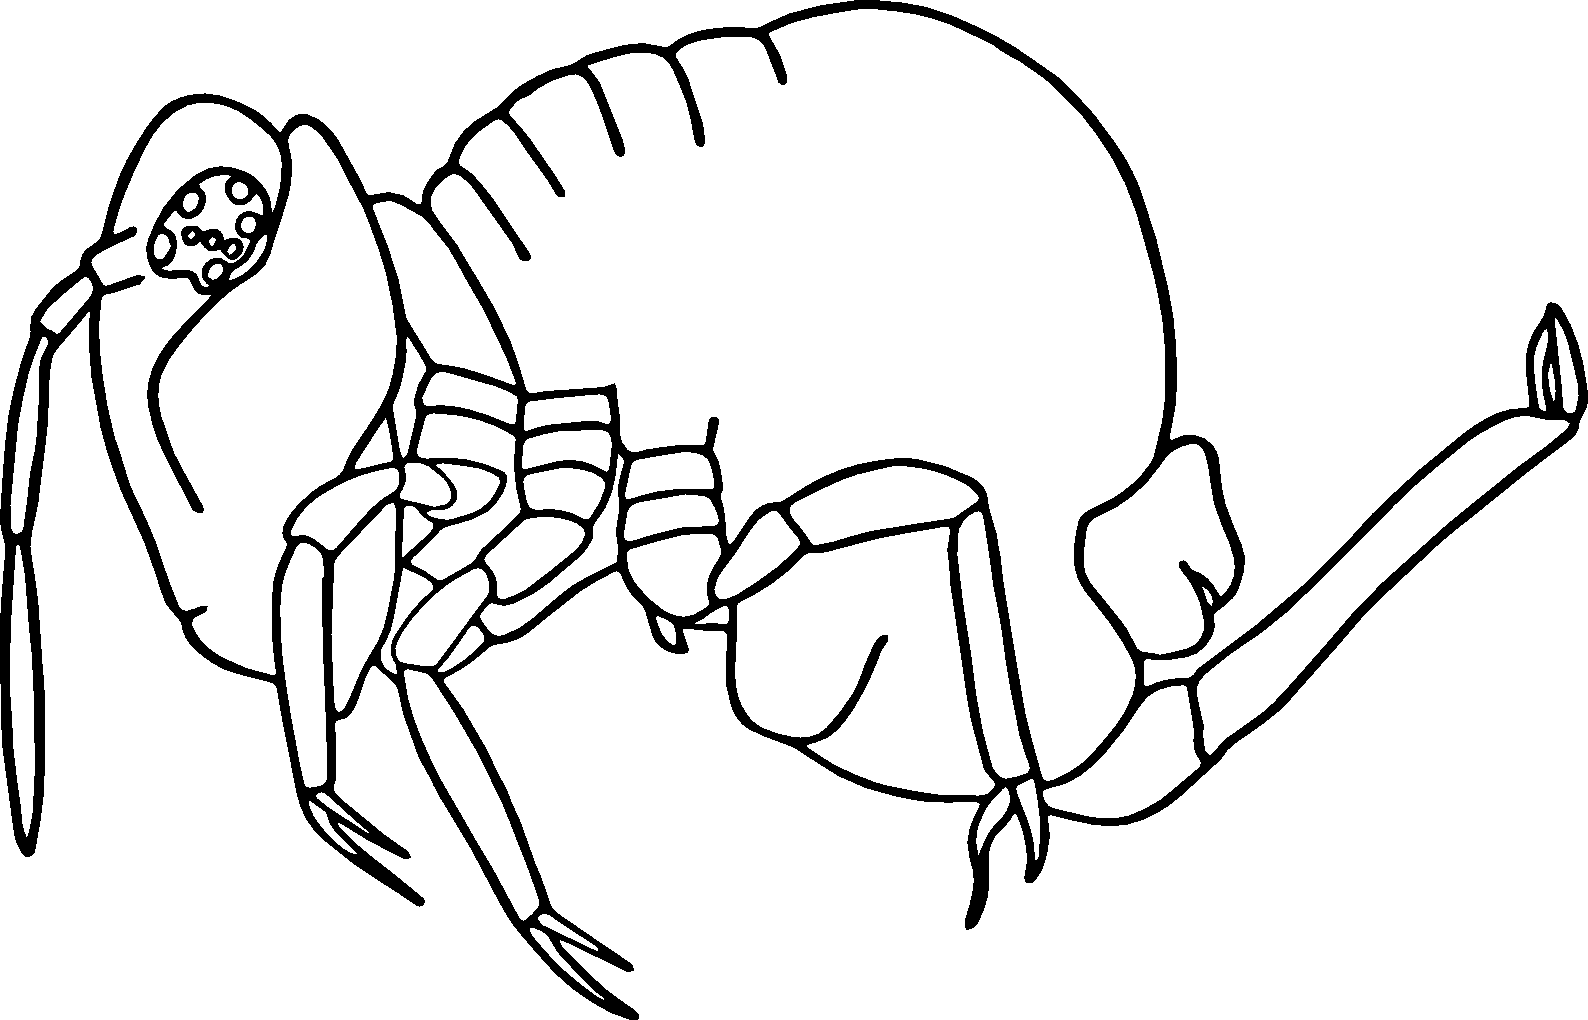
\includegraphics[width=0.4\textwidth]{nonpterygote/sminthuridHabitus}}
  \caption{Symphypleona (Sminthuridae) habitus \citep[redrawn from][Fig. 19]{bhlitem30465Insects}}
  \label{fig:sminthhab}
\end{figure}

\subsubsection{Poduromorpha}\index{Poduromorpha}
\noindent{}\textit{Diagnostic characters:} Head typically prognathous, not anteroposteriorly flattened; antennae usually shorter than head; prothorax distinct dorsally, broadly articulated with head; legs relatively short; abdominal segments 2--4 not fused.\vspace{3mm}

\noindent{}\textit{Natural History:} Like Symphypleona, these hexapods are biologically diverse, with many semiaquatic species. There are also about 10 families.\vspace{3mm}

\begin{figure}[ht!]
  \centering
    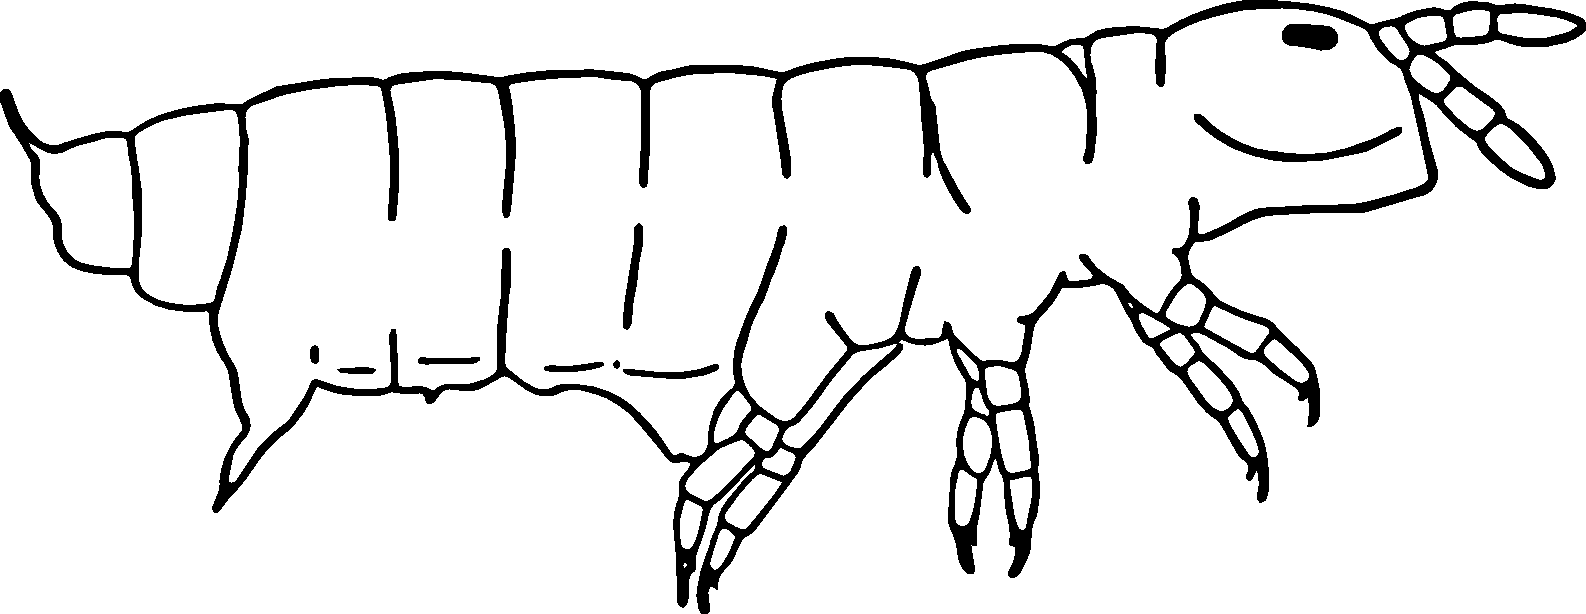
\includegraphics[width=0.4\textwidth]{nonpterygote/hypogastruridHabitus}
  \caption{Poduromorpha (Hypogastruridae) habitus \citep[redrawn from][Fig. 14]{bhlitem30465Insects}}
  \label{fig:hypogasthab}
\end{figure}

\subsubsection{Entomobryomorpha}\index{Entomobryomorpha}
\noindent{}\textit{Diagnostic characters:} Head hypognathous to prognathous, not anteroposteriorly flattened; antennae longer than head; prothorax indistinct dorsally, narrowly articulated with head; abdominal segments 2--4 not fused; body and legs relatively long, thin.\vspace{3mm}

\noindent{}\textit{Natural History:} There are about 8 extant families \citep{SotoAdames501}. Entomobryidae and Tomoceridae are frequently collected in the eastern USA in leaf litter.\vspace{3mm}

\begin{figure}[ht!]
  \centering
    \reflectbox{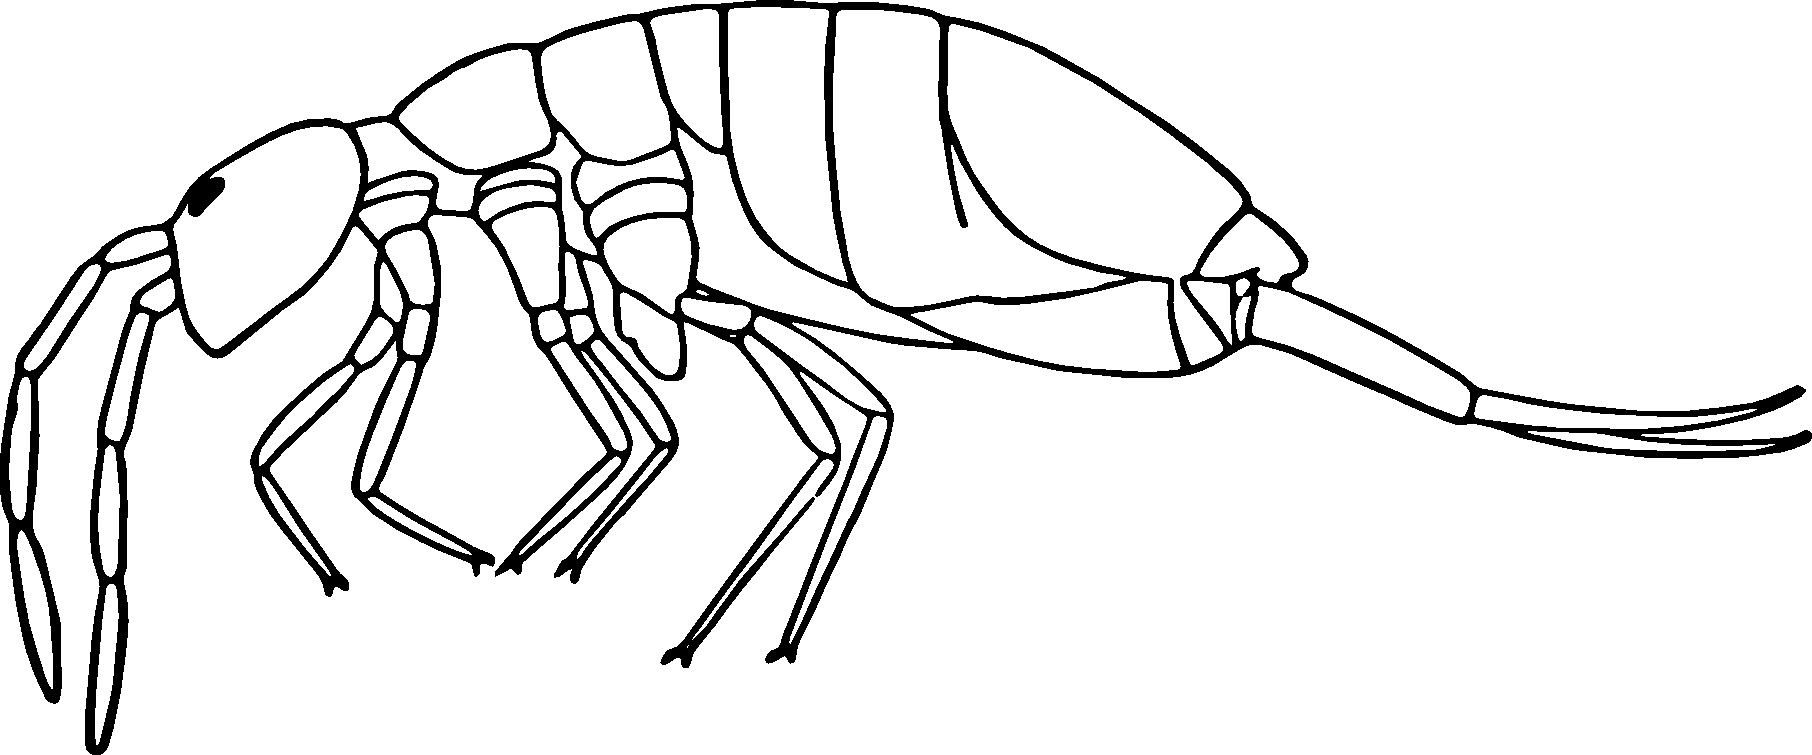
\includegraphics[width=0.5\textwidth]{nonpterygote/entomobryidHabitus.pdf}}
  \caption{Entomobryomorpha (Entomobryidae) habitus \citep[redrawn from][Fig. 17]{bhlitem30465Insects}}
  \label{fig:entomobry}
\end{figure}

\begin{figure}[ht!]
  \centering
    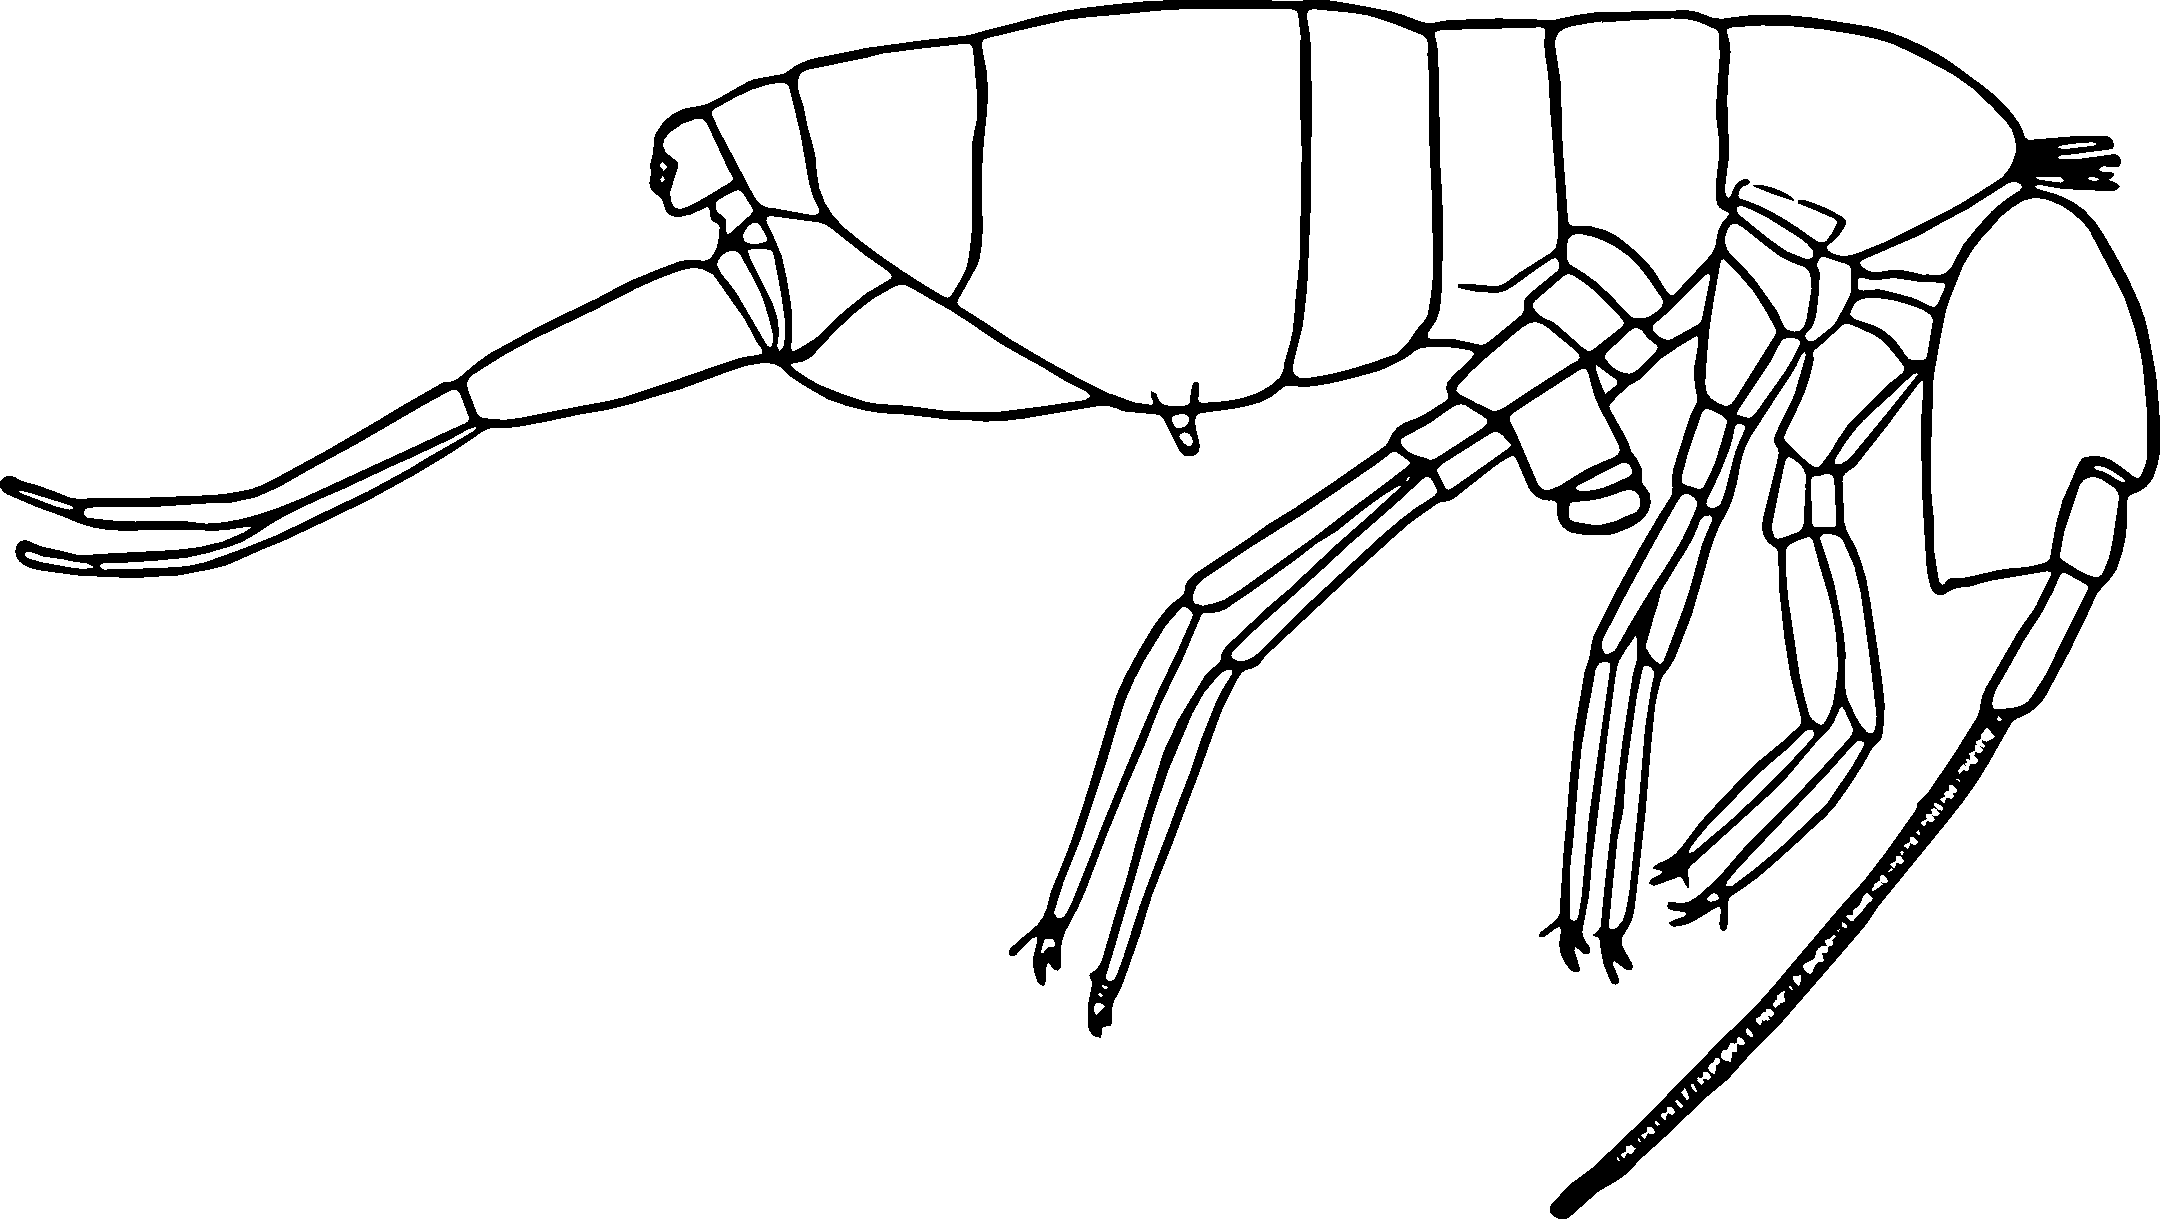
\includegraphics[width=0.45\textwidth]{nonpterygote/tomoceridHabitus}
  \caption{Tomoceridae habitus \citep[redrawn from][Fig. 16]{bhlitem30465Insects}}
  \label{fig:tomocer}
\end{figure}

\section*{Insecta}\index{Insecta}
The remaining arthropods we will examine in lab are true insects. In addition to many internal characters we won't examine (\textit{e.g.}, Johnston's organ) insects can be recognized by:
\begin{itemize}
\item Antennae 3-segmented (\textit{i.e.}, segments with intrinsic musculature), with apical segment (flagellum) usually subdivided
\item Mouthparts not usually enveloped by cuticular evagination (\textit{i.e.}, insects are \textit{ectognathous})
\item Ovipositor present
\end{itemize}

\section{Archaeognatha (Microcoryphia, bristletails)}\index{Archaeognatha}
\noindent{}\textit{Diagnostic characters:} Compound eyes well-developed, adjacent dorsally; maxillary palps longer than legs, subdivided into 7 annuli; labial palps subdivided into 3 annuli; meso- and metacoxa with styli present; styli present on abdominal segments 2--9; abdomen with 3 scaly appendages present apically (2 cerci, 1 terminal appendage); body ``humpbacked'', scaly; paired eversible vesicles usually present on abdominal segments 1--7.\vspace{3mm}

\noindent{}\textit{Natural History:} These insects are frequently found on or around fallen logs and rocks, where they survive on algae, lichens, and decaying matter. There are about 350 known species, in 2 families.\vspace{3mm}

\begin{figure}[ht!]
  \centering
    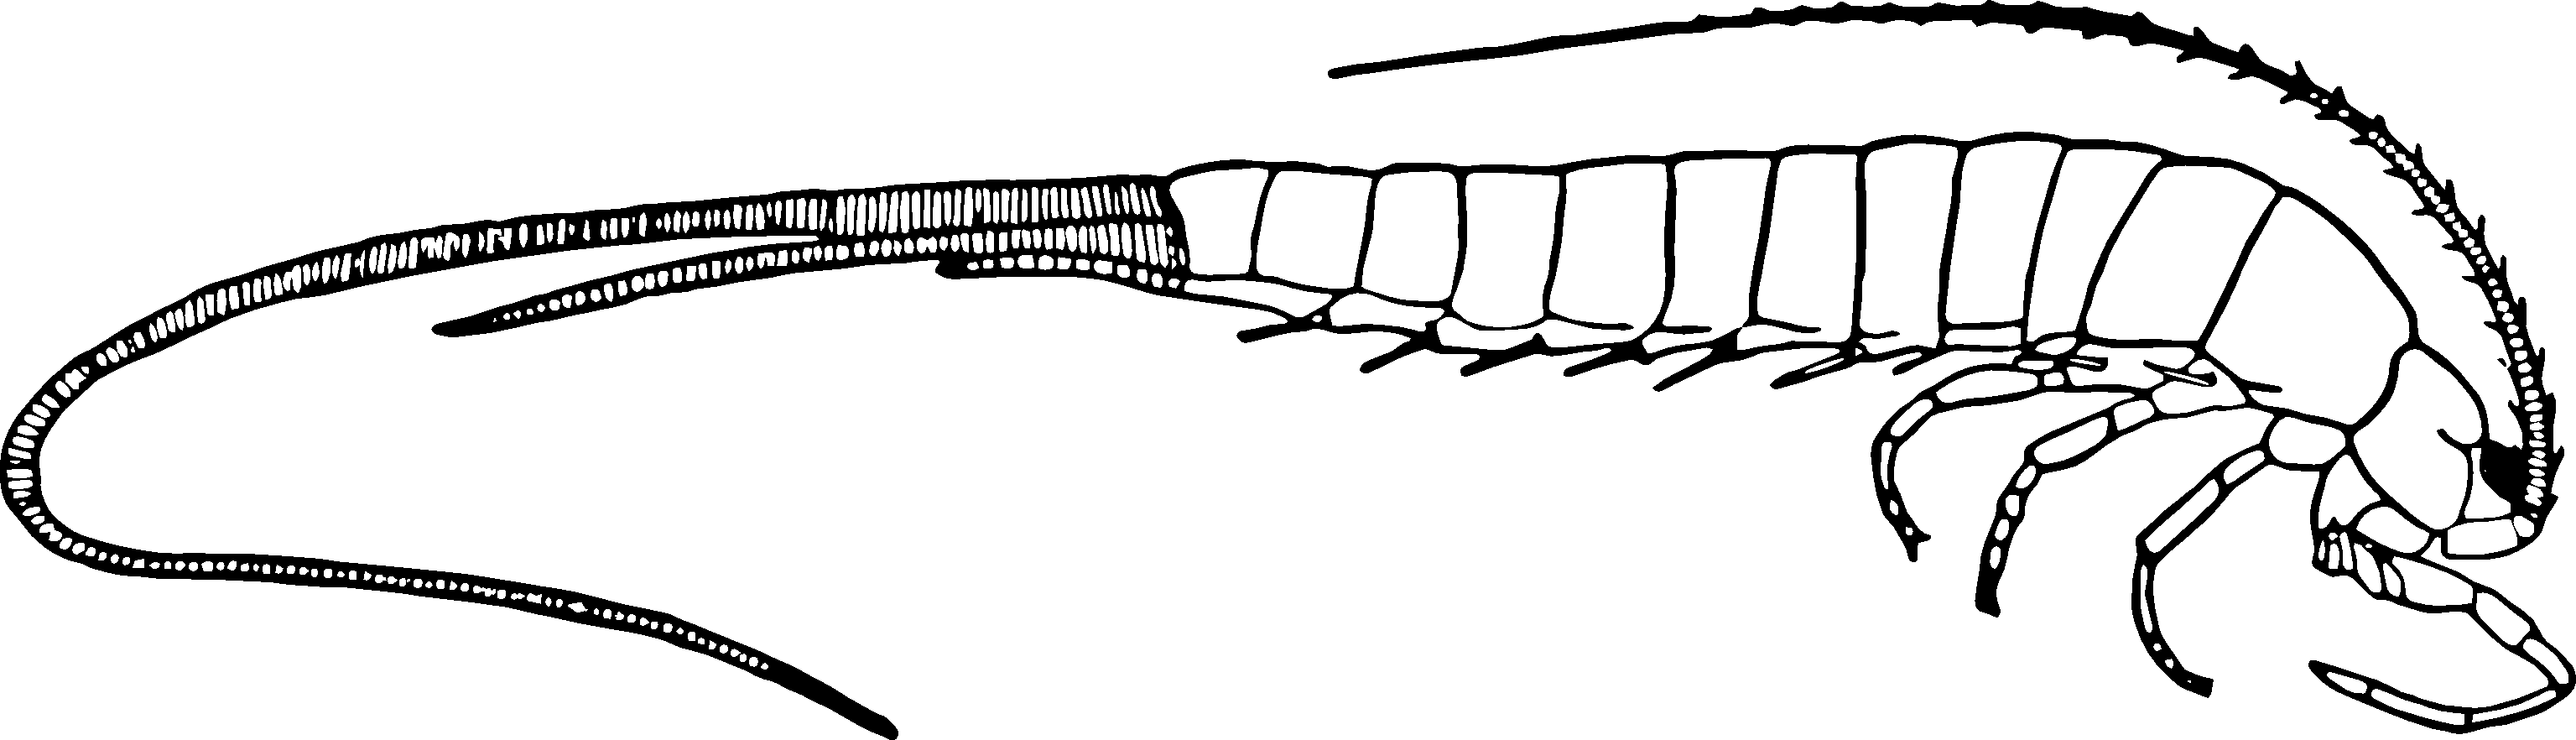
\includegraphics[width=0.7\textwidth]{nonpterygote/archaeognathHabitus}
  \caption{Archaeognathan lateral habitus \cite[redrawn from][Fig. 1]{bhlitem30465Insects}}
  \label{fig:archhabit}
\end{figure}

\begin{figure}[ht!]
  \centering
    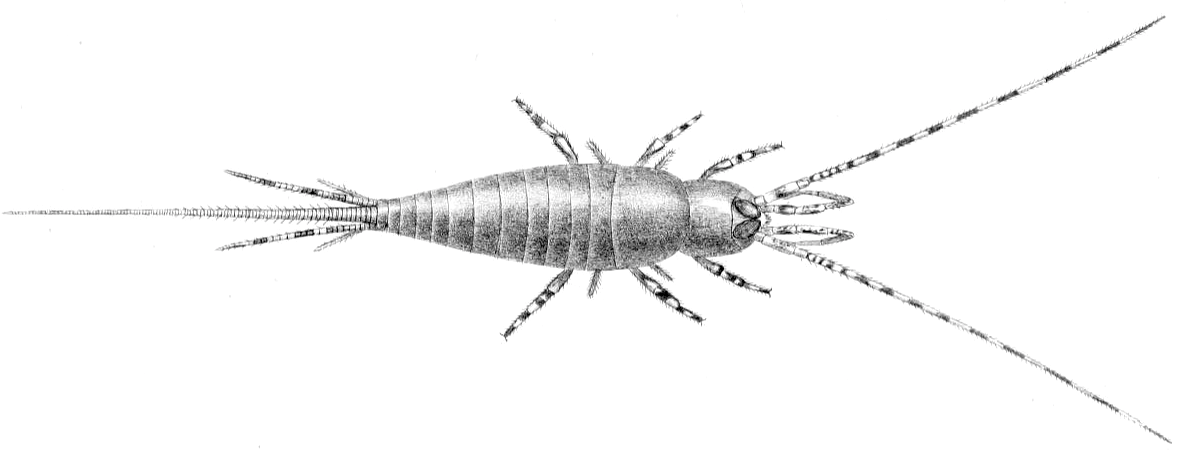
\includegraphics[width=0.8\textwidth]{nonpterygote/archaeoHab2}
  \caption{Archaeognathan dorsal habitus \citep[][Plate 53]{bhlitem43892Lubbock}}
  \label{fig:archhead}
\end{figure}

\begin{theo}
{}Which characteristics would you interpret as ancestral? Can you find evidence that insects are related to other pancrustaceans?\vspace{3mm}

\noindent{}Have you seen these insects move? Why do they have a ``humpbacked'' habitus? Can you find and draw the styli? What might these be remnants of? \end{theo}

\section{Zygentoma (``Thysanura'', in part; silverfish, firebrats)}\index{Zygentoma}

\noindent{}\textit{Diagnostic characters:} Compound eyes small, widely separated; maxillary palps shorter than legs, subdivided into 6 annuli; labial palps subdivided into 4 annuli; styli on meso- and metacoxa absent, usually present on abdominal segments 2--9; abdomen with 3 bare appendages present apically (2 cerci, 1 terminal appendage); body dorsoventrally flattened, scaly; paired eversible vesicles usually present on abdominal segments 1--7.\vspace{3mm}

\noindent{}\textit{Natural History:} Zygentoma is about as diverse as Archaeognatha. Many species inhabit buildings, where they can be pests (eating paper, glue, and other starchy products). Some species live in ant nests, and many can digest cellulose and lignin.\vspace{3mm}

\begin{figure}[ht!]
  \centering
    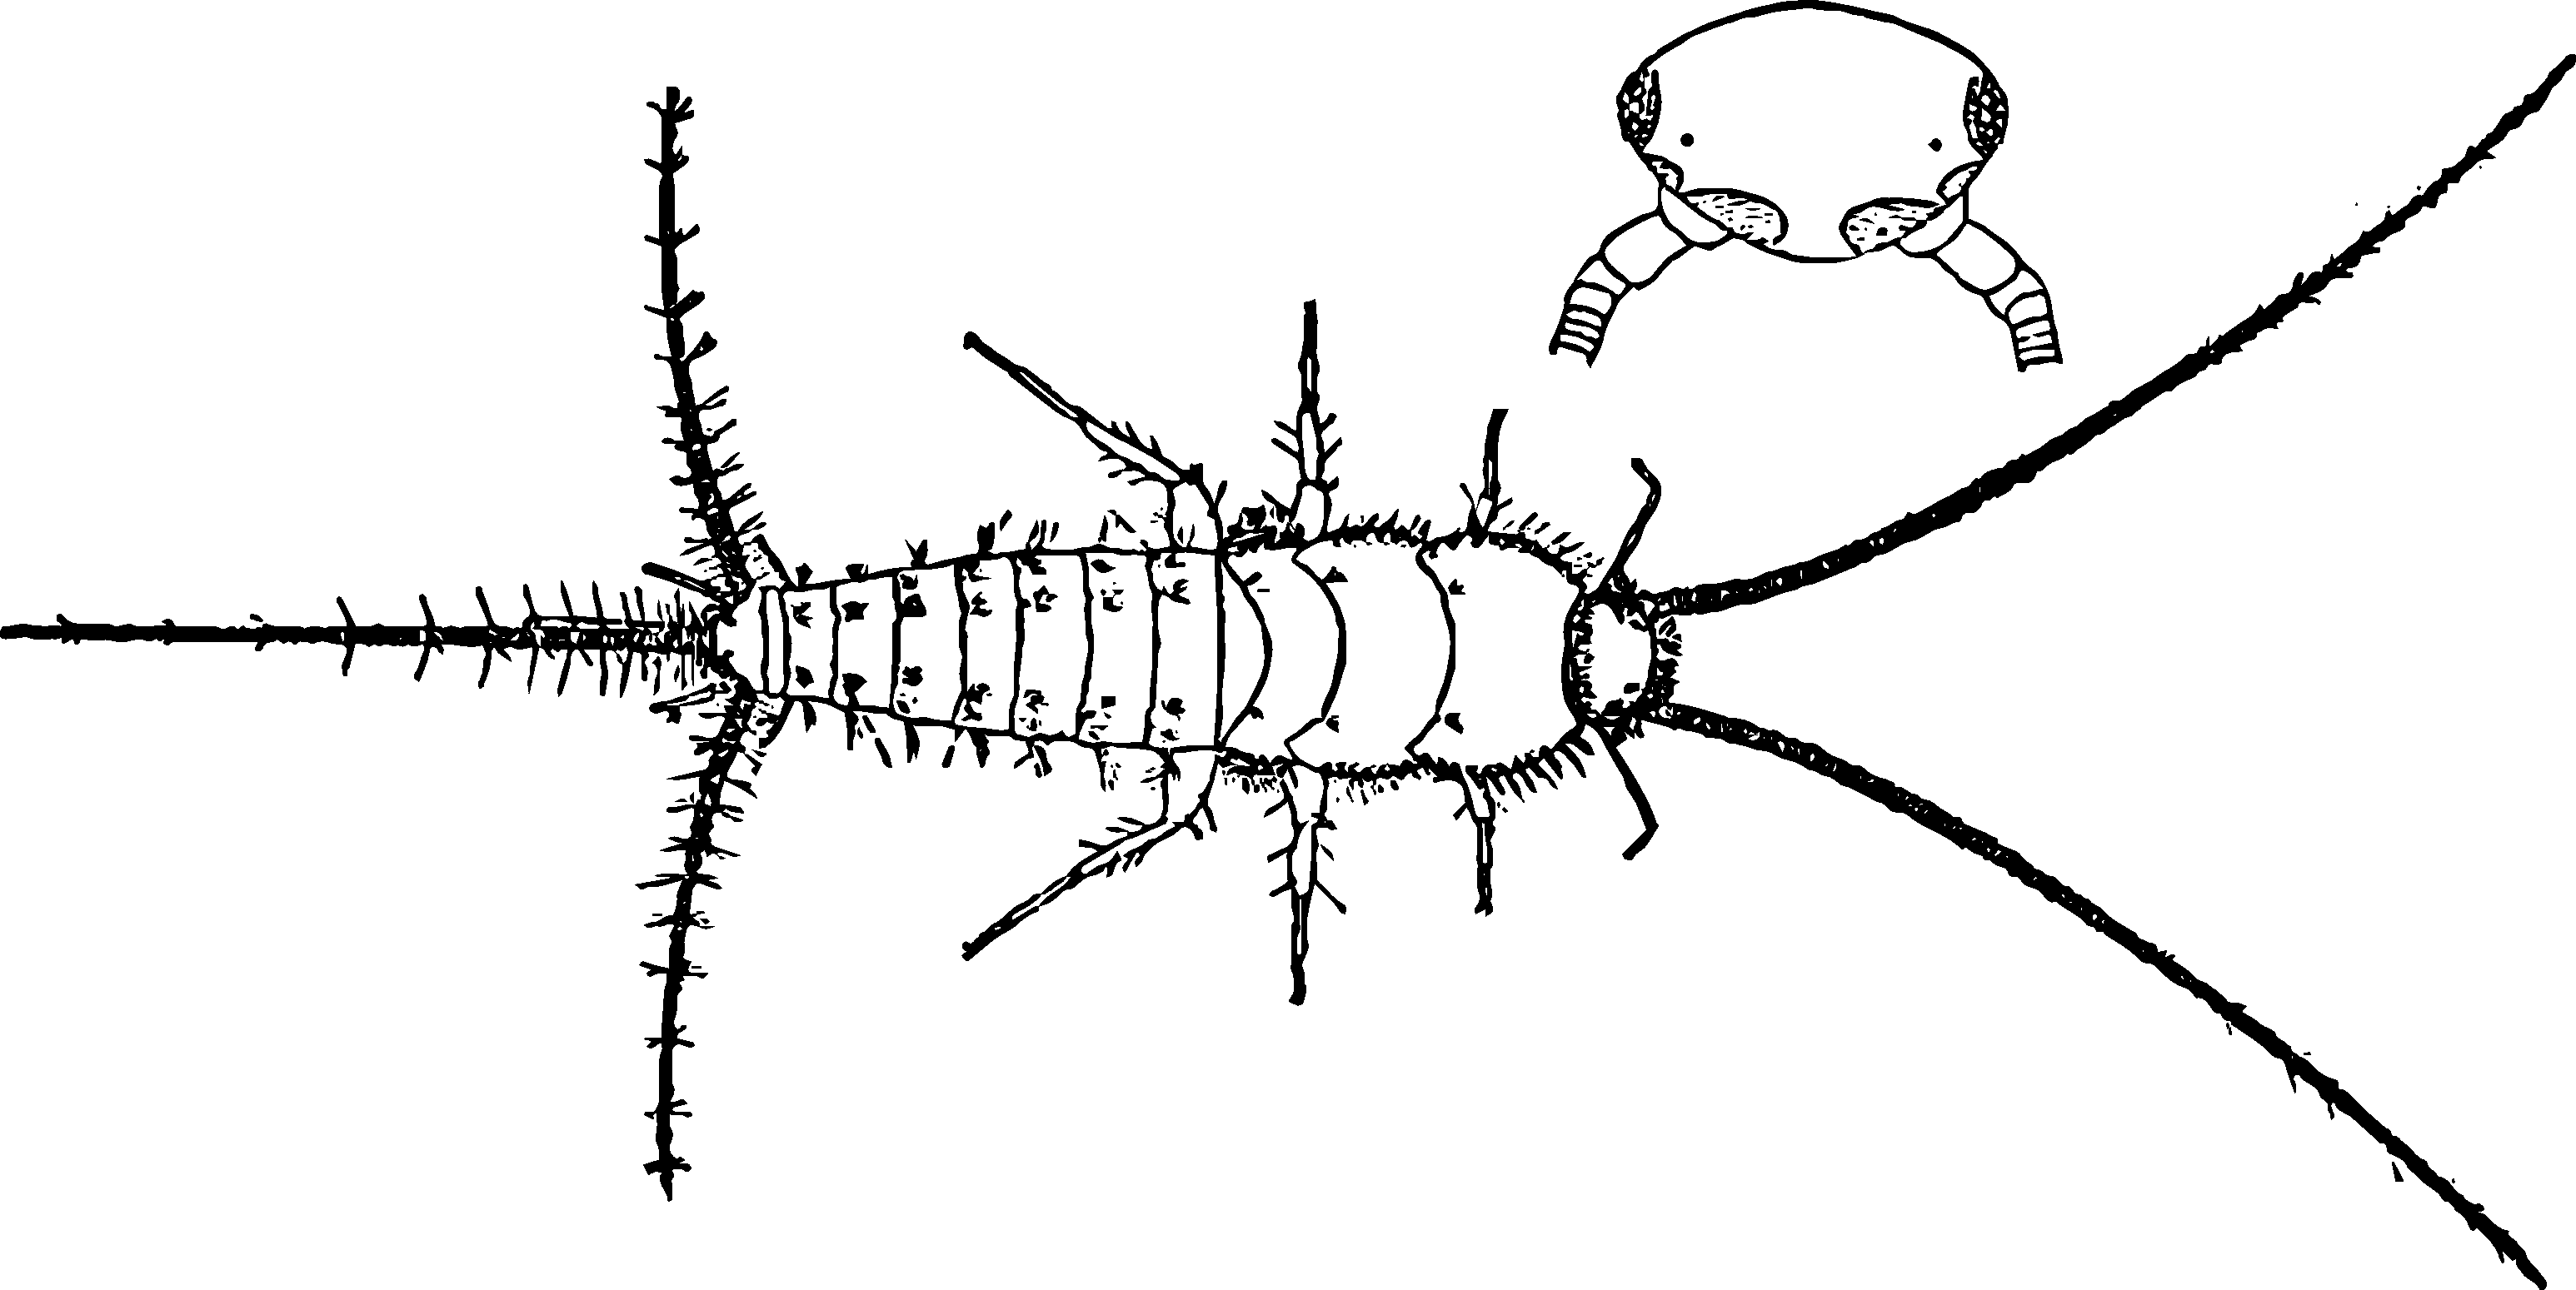
\includegraphics[width=0.8\textwidth]{nonpterygote/lepismatidHabitus}
  \caption{Zygentoma dorsal habitus and head (inset) \citep[redrawn from][Figs. 1, 10]{bhlpart1409lepismat}}
  \label{fig:zygenhabit}
\end{figure}

\begin{figure}[ht!]
  \centering
    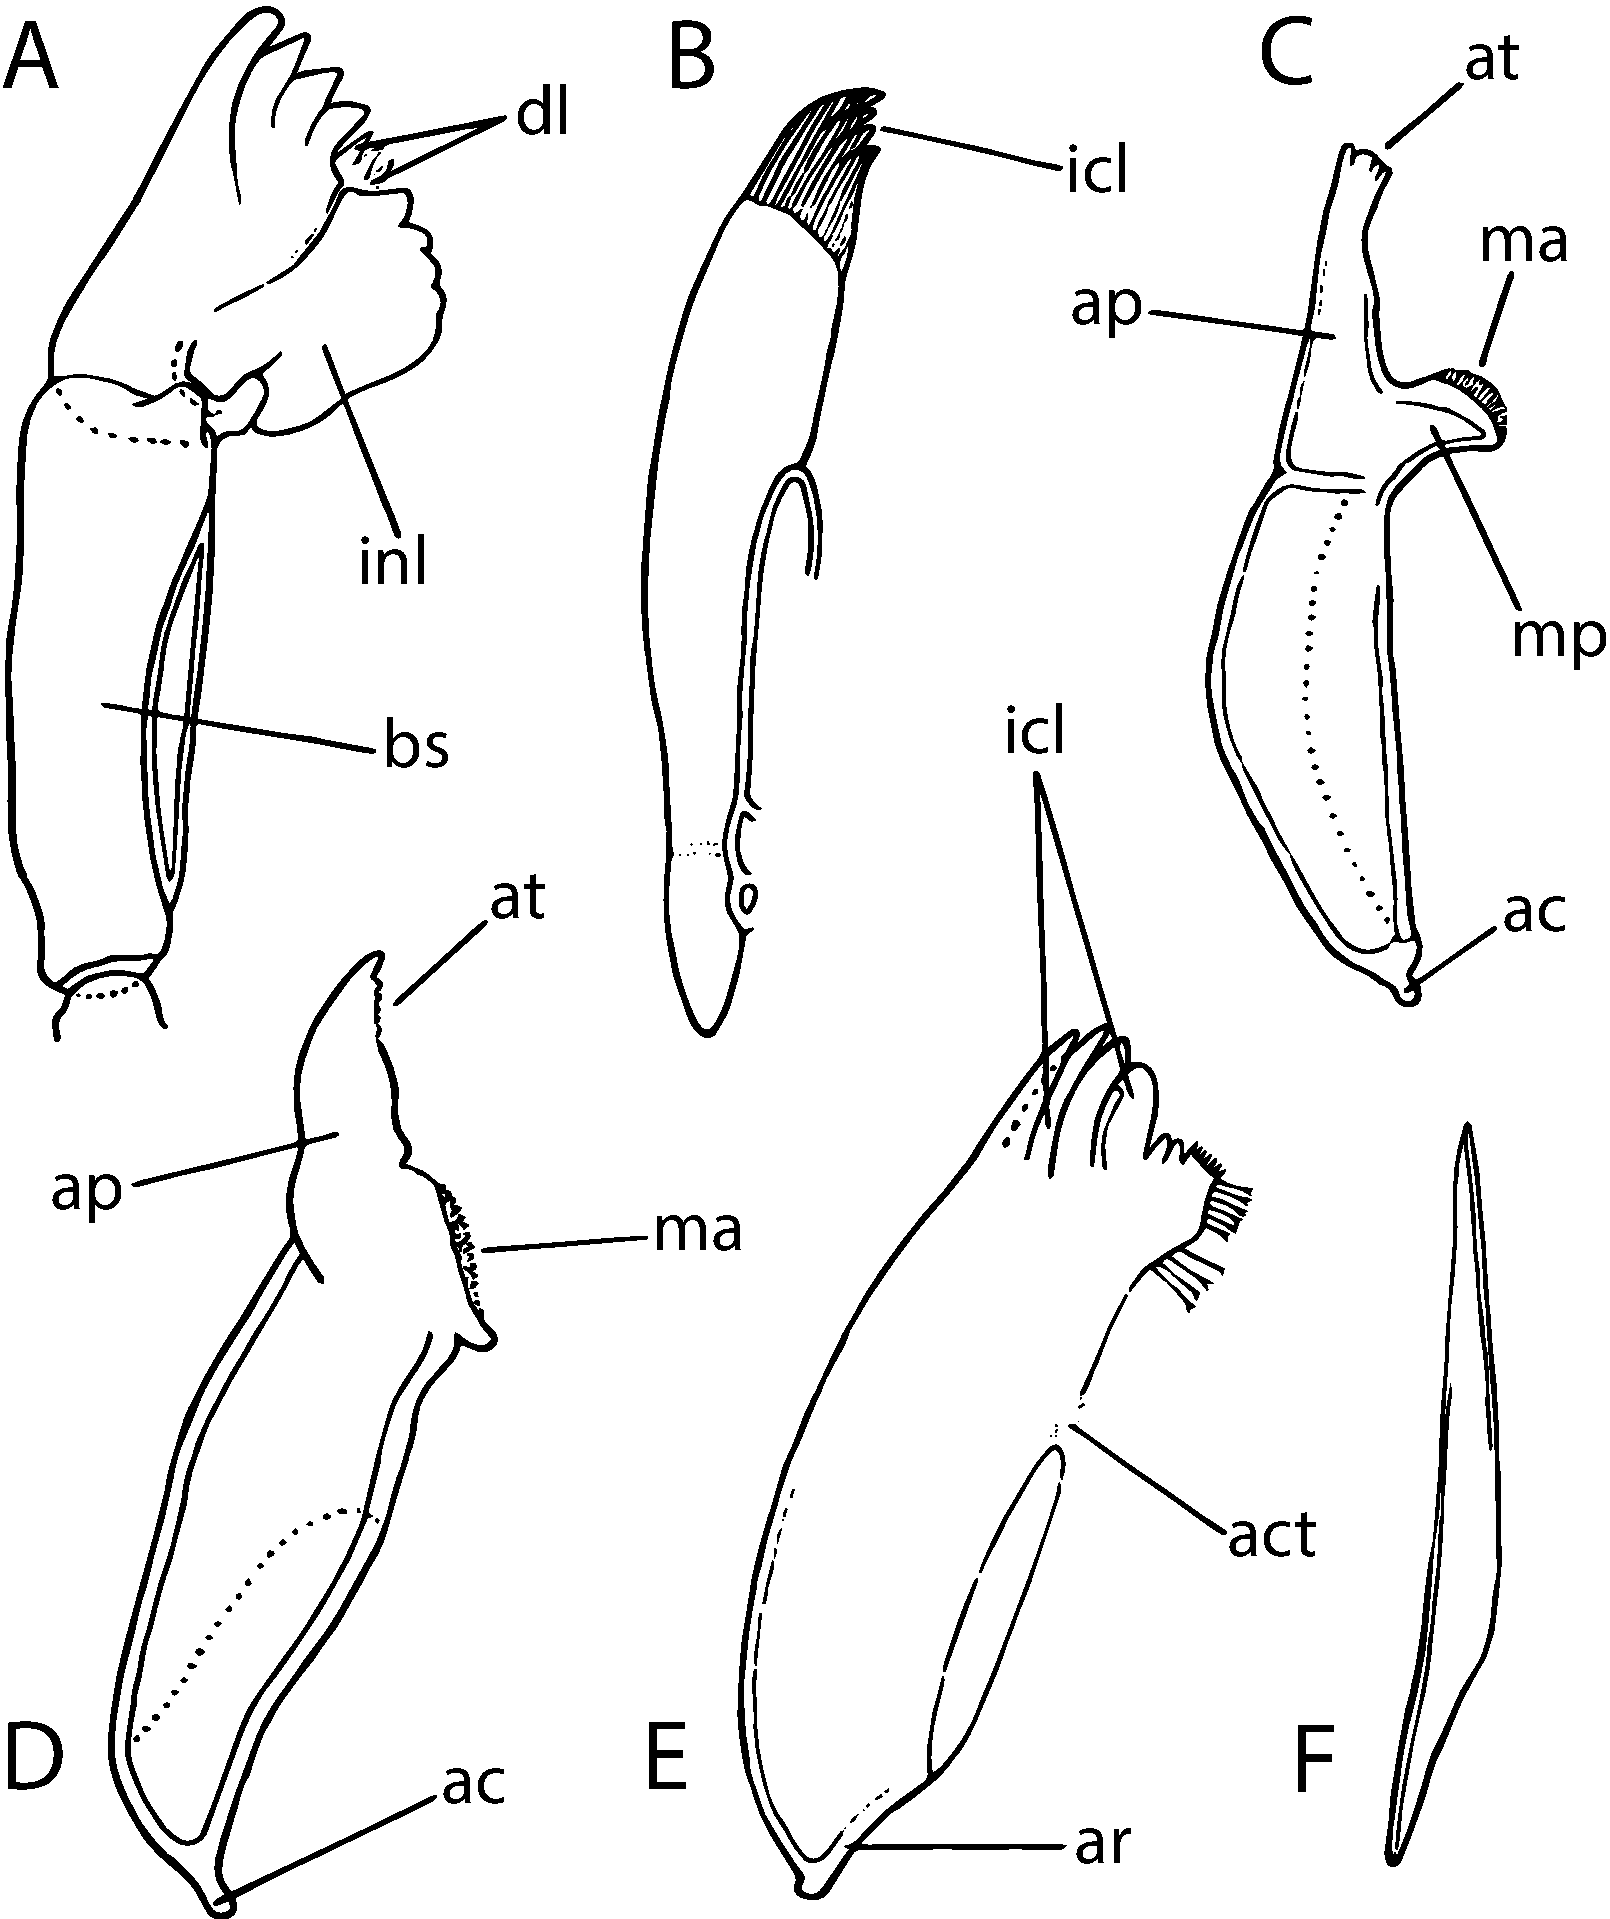
\includegraphics[width=0.55\textwidth]{nonpterygote/mandibles.pdf}
  \caption{Mandibles of Symphyla and Apterygota in dorsal view. (A) Myriapoda: Symphyla; (B) Japygidae; (C) Archaeognatha; (D) Collembola; (E) Zygentoma; (F) Protura. Abbreviations: ac=articulating condyle; act=acetabulum; ap=apical process; ar=articulating ridge; at=apical teeth; bs=basal segment; dl=dentate lamella; id=incisor lobe; inl=inner lobe; ma=molar area; mp=molar process; ol=outer lobe \citep[redrawn from][Fig. 1]{bhlpart81512}}
  \label{fig:mandibles}
\end{figure}

\begin{theo}
{}As stated above, Insecta have three traits that set them apart from previous taxa we examined: \textbf{(1)} 3-segmented antenna, with Johnston's organ in the pedicel; \textbf{(2)} exposed mouthparts and a transition to dicondylous mandibles (figures \ref{fig:mandibles}B and F vs. E); \textbf{(3)} presence of ovipositor. Can you describe the adaptive nature of these traits and how they may have contributed to the extraordinary diversity of Insecta?
\end{theo}

\clearpage
\thispagestyle{empty}
